In figure \ref{1realiz5yr} one realization of $\{X(t): t \in [0,1825]\}$ is shown. It is not possible to tell much about the general tendencies from this single realization, however we can see that the individual experienced two heavy and some light infections over the course of five years. The proportion of time spent in each state seems to correspond well to the results found in \textbf{b}, stating that an individual is  $92.33\%$, lightly infected $5.82\%$ and heavily infected $1.85\%$ of the time. 

\begin{figure}
    \centering
    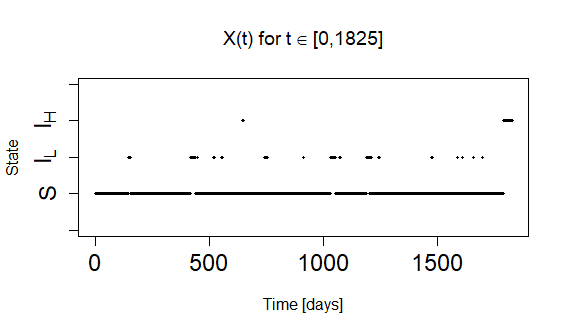
\includegraphics[width=130mm]{1real5yr.png}
    \caption{One realization of the continuous-time Markov chain $\{X(t):t \in [0, 1825]\}$.}
    \label{1realiz5yr}
\end{figure}

